The viewer layer makes up the UI of Project Iris. It will expose settings and raw data to the user to facilitate a better understanding of what is taking place behind the scenes.

\begin{figure}[h!]
	\centering
	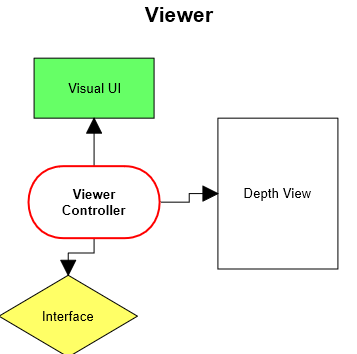
\includegraphics[width=0.60\textwidth]{images/viewer}
	\caption{Example subsystem description diagram}
\end{figure}

\subsection{Visual UI}
The visual UI is the main component of Project Iris that a user will see. It allows the user to change mode, calibrate the software, and see the raw data generated by the software. All changes will then go through the controller.

\subsubsection{Assumptions}
The UI will be built using windows 10 APIs.

\subsubsection{Subsystem Interfaces}

\begin {table}[H]
\caption {Subsystem interfaces} 
\begin{center}
    \begin{tabular}{ | p{1cm} | p{6cm} | p{3cm} | p{3cm} |}
    \hline
    ID & Description & Inputs & Outputs \\ \hline
    \#1 & UI/Controller & \pbox{3cm}{Device Data\\Software State} & \pbox{3cm}{User Selections}  \\ \hline
    \end{tabular}
\end{center}
\end{table}

\subsection{Viewer Controller}
The controller is where an algorithms or data changes the UI needs to make are accomplished. This will facilitate seperating the Windows UI elements from the rest of Project Iris and should improve the ability of the project to be ported later.

\subsubsection{Responsibilities}
This subsystem is responsible for updating the Tracking layer, calling the calibration utility, and ensuring important events are relayed to the user.

\subsubsection{Subsystem Interfaces}

\begin {table}[H]
\caption {Subsystem interfaces} 
\begin{center}
	\begin{tabular}{ | p{1cm} | p{6cm} | p{3cm} | p{3cm} |}
		\hline
		ID & Description & Inputs & Outputs \\ \hline
		\#1 & Controller/UI & \pbox{3cm}{User Selections} & \pbox{3cm}{Device Data \\Software State}  \\ \hline
		\#2 & Viewer interface & \pbox{3cm}{Device Data\\System Events\\Software State} & \pbox{3cm}{Settings Changes\textsl{}}  \\ \hline
	\end{tabular}
\end{center}
\end{table}
